% Beamer presentation
\documentclass[11pt,aspectratio=43,ignorenonframetext,t]{beamer}

% Presentation settings
\mode<presentation>{
  \usetheme[framenumber,titleframestart=1]{UoM_alex}
  \usefonttheme{professionalfonts} % using non standard fonts for beamer
  \usefonttheme{serif}
  \usepackage{fontspec}
  \setmainfont[Ligatures=TeX]{Arial}
}

% Handout settings
\mode<article>{
  \usepackage{fullpage}
  \usepackage{fontspec}
  \setmainfont[Ligatures=TeX]{Arial}
  \setlength{\parskip}{1.5\baselineskip} % correct beamer line spacings
  \setlength{\parindent}{0cm}
  \usepackage{enumitem}
  \setlist[itemize]{topsep=0pt}
}

 % Packages
\usepackage{graphicx}
\graphicspath{{./images/png}} % generic graphics path; overridden if necessary
\usepackage{amsmath}
\allowdisplaybreaks[1] % allow eqnarrays to break across pages
\usepackage{amssymb} 
\usepackage[HTML]{xcolor}
\definecolor{uomlinkblue}{HTML}{0071BC}
\usepackage{hyperref}
\hypersetup{
  colorlinks=true,
  linkcolor=uomlinkblue,
  filecolor=uomlinkblue,      
  urlcolor=uomlinkblue,
  pdflang={en-GB},
}
\usepackage[document]{ragged2e} % left aligned text for accessibility
\usepackage{tikz}
\usetikzlibrary{positioning, arrows, arrows.meta}
\usepackage{unicode-math} % unicode maths for accessibility
\usepackage{pdfcomment}   % for alt text for accessibility
\usepackage{rotating}     % allow portrait figures and tables
\usepackage{subfigure}    % allow matrices of figures
\usepackage{float}        % allows H option on floats to force here placement
\usepackage{multirow}     % allows merging of rows in tables
\usepackage{tabularx}     % allows fixed width tables
\usepackage{ctable}       % modifies \hline for use in table
\usepackage{bm}           % allow bold fonts in equations
\usepackage{pgf}          % allow graphics manipulation
\usepackage{etoolbox}
  
% Custom commands
\newcolumntype{Z}{>{\centering\arraybackslash}X}  % tabularx centered columns 

\makeatletter
  \DeclareRobustCommand{\em}
  {
    \@nomath\em
    \if b
      \expandafter\@car\f@series\@nil \normalfont
    \else
      \bfseries
    \fi
  }
\makeatother

\makeatletter
  \preto{\@verbatim}{\topsep=0pt \partopsep=0pt}
\makeatother

\def\checkmark{
  \tikz\fill[scale=0.4](0,.35) -- (.25,0) -- (1,.7) -- (.25,.15) -- cycle;
}

% Counters
\newcounter{example_number} % keep track of the example questions

% Frontmatter
\newcommand{\cmclecture}[1]{
  \title{Combinatorial Mesh Calculus (CMC): Lecture #1}
}
\author{
  Lectured by:
  \href{https://scholar.google.com/citations?user=x4R-snQAAAAJ&hl=en}
  {Dr. Kiprian Berbatov}$^1$\\
  \smallskip
  Lecture Notes Compiled by:
  \href{https://scholar.google.com/citations?user=CoIpITkAAAAJ&hl=en}
  {Muhammad Azeem}$^1$\\
  \smallskip
  Under the supervision of:
  \href{https://scholar.google.co.uk/citations?user=3nWJe5wAAAAJ&hl=en}
  {Prof. Andrey P. Jivkov}$^1$\\
  \smallskip
  {\tiny $^1$Department of Mechanical and Aerospace Engineering,
    The University of Manchester, Oxford Road, Manchester M13 9PL, UK}
}

% Special frames
\newcommand{\cmctitleframe}{
  \titlepage
  \begin{tikzpicture}[remember picture,overlay]
    \node[anchor=south east] at (current page.south east) {
      \href{https://youtube.com/@kipi.berbatov}{
        
\includegraphics[width=1.5cm]{youtube-icon.png}
      }
    };
  \end{tikzpicture}
}
\newcommand{\cmcendframe}{
  \begin{figure}
    \centering
    
\includegraphics[width=0.85\linewidth]{Thanks.png}
  \end{figure}
}

\cmclecture{2}
\date{15 October 2025}

\begin{document}

%========================= TITLE =========================
\begin{frame}
  \cmctitleframe
\end{frame}

\begin{frame}{Definition of an n–ary Operation}
\begin{block}{Definition.}  
Let \( X \) be a nonempty set and \( n \in \mathbb{N} \).  
An \emph{n–ary operation} on \( X \) is a function
\[
f : X^n \longrightarrow X.
\]  
\end{block}

\begin{block}{Special cases:}
\begin{itemize}
  \item \( n = 0 \): a \emph{nullary operation} (a constant \( c \in X \)).
  \item \( n = 1 \): a \emph{unary operation} \( f: X \to X \).
  \item \( n = 2 \): a \emph{binary operation} \( f: X \times X \to X \).
\end{itemize}

\textbf{Notation:} For a binary operation, we often write  
\[
f(x,y) = x * y.
\]
    
\end{block}
\end{frame}

% ============================================================
\begin{frame}{Examples of n–ary Operations}
\vspace{-0.3cm}
Let \( X = \mathbb{Z} \).

\textbf{Nullary (0–ary):}
\[
c = 0 \in \mathbb{Z}.
\]
\textbf{Unary (1–ary):}
\[
f_1(x) = -x, \quad f_2(x) = x + 1, \quad f_3(x) = \frac{1}{x^2 + 1}.
\]
Each maps \( \mathbb{Z} \to \mathbb{Z} \) or \( \mathbb{R} \to \mathbb{R} \).

\textbf{Binary (2–ary):}
\[
f_1(x,y) = x + y, \quad f_2(x,y) = xy, \quad f_3(x,y) = x^y.
\]

\textbf{Check closure:}
\begin{itemize}
  \item \(x+y \in \mathbb{Z}\): $\checkmark$ binary operation on \(\mathbb{Z}\).
  \item \(xy \in \mathbb{Z}\): $\checkmark$ binary operation.
  \item \(x^y\) may not be integer for all \(x,y\in\mathbb{Z}\) (e.g.\ \(x=-1, y=\frac12\)), so $\times$, not closed on \(\mathbb{Z}\).
\end{itemize}
\end{frame}

% ============================================================
\section{Properties of Binary Operations}
% ============================================================

\begin{frame}{Associativity and Commutativity}
\vspace{-0.3cm}
Let \( *: X\times X \to X \) be a binary operation.

\textbf{Definition (Associativity):}
\[
a * (b * c) = (a * b) * c, \quad \forall a,b,c \in X.
\]

\textbf{Definition (Commutativity):}
\[
a * b = b * a, \quad \forall a,b \in X.
\]

\begin{center}
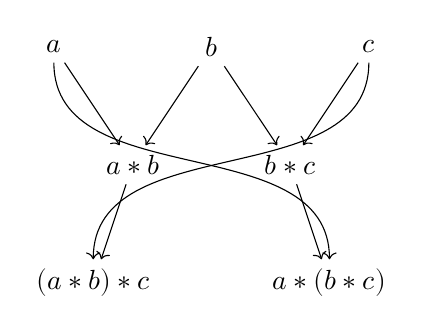
\begin{tikzpicture}[scale=1.0]
% Top row
\node (a) at (0,0) {$a$};
\node (b) at (2,0) {$b$};
\node (c) at (4,0) {$c$};

% Middle row
\node (ab) at (1,-1.5) {$a*b$};
\node (bc) at (3,-1.5) {$b*c$};

% Bottom row
\node (abc1) at (0.5,-3) {$(a*b)*c$};
\node (abc2) at (3.5,-3) {$a*(b*c)$};

% Arrows from top to middle
\draw[->] (a) -- (ab);
\draw[->] (b) -- (ab);
\draw[->] (b) -- (bc);
\draw[->] (c) -- (bc);

% Arrows from middle to bottom
\draw[->] (ab) -- (abc1);
\draw[->] (c) to[out=-90, in=90] (abc1);
\draw[->] (a) to[out=-90, in=90] (abc2);
\draw[->] (bc) -- (abc2);
\end{tikzpicture}
\end{center}
\end{frame}

\begin{frame}{Example}

\begin{block}{}
    \begin{itemize}
  \item On \((\mathbb{Z}, +)\): addition is both \textbf{associative} and \textbf{commutative}, since for all \(a,b,c \in \mathbb{Z}\),
  \[
  (a+b)+c = a+(b+c), \qquad a+b = b+a.
  \]
  \item On \((\mathbb{R}, -)\): subtraction is \textbf{neither associative nor commutative}, e.g.
  \[
  (5-3)-2 = 0 \neq 5-(3-2)=4, \quad 5-3 \neq 3-5.
  \]
  \item On \((\mathbb{R}, \times)\): multiplication is \textbf{associative and commutative}, since
  \[
  (a b)c = a(b c), \qquad a b = b a.
  \]
\end{itemize}
\end{block}
\end{frame}

\begin{frame}{Example}
\begin{block}{}
\begin{itemize}
  \item On \((M_{2\times2}(\mathbb{R}), \times)\): matrix multiplication is \textbf{associative} but \textbf{not commutative}; for example,
  \[
  A=\begin{bmatrix}1&0\\0&0\end{bmatrix},\ 
  B=\begin{bmatrix}0&1\\0&0\end{bmatrix} 
  \implies AB\neq BA.
  \]
  \item On \((\mathbb{R}, \div)\): division is \textbf{neither associative nor commutative}, e.g.
  \[
  (8\div4)\div2 = 1 \neq 8\div(4\div2)=4.
  \]
  \item On the set of functions \(F(X)\) with pointwise addition \((f+g)(x)=f(x)+g(x)\): operation is both \textbf{associative} and \textbf{commutative}.
\end{itemize}
\end{block}

\end{frame}

% ============================================================
\begin{frame}{Identity (Neutral) Elements}
\begin{block}{Definition.}  
Let \((X,*)\) be a set with a binary operation.  
An element \(e \in X\) is called a
\begin{itemize}
  \item \textbf{left identity} if \( e * x = x \) for all \(x\in X\),
  \item \textbf{right identity} if \( x * e = x \) for all \(x\in X\),
  \item \textbf{two–sided identity (neutral element)} if both hold.
\end{itemize}
\end{block}


\begin{block}{Remark}
If both left and right identities exist, they are necessarily equal (proved later).
\end{block}

\end{frame}

\begin{frame}{Examples}
\vspace{-0.3cm}
\begin{block}{}
\begin{itemize}
    \item \textbf{Example:} $(\mathbb{N}, +): \; e = 0; \quad (\mathbb{R}, \times): \; e = 1.$\\
    \item \textbf{Counterexample:} Consider the operation \((-)\) on the real numbers \(\mathbb{R}\), defined by $a * b = a - b.$
We want to check whether there exists an element \(e \in \mathbb{R}\) such that
\[
a - e = a = e - a, \quad \forall\, a \in \mathbb{R}.
\]
The first equation \(a - e = a\) implies \(e = 0\).  
Substituting \(e = 0\) into the second equation gives \(e - a = 0 - a = -a\).  
For this to equal \(a\) for all \(a\), we would need \(-a = a\), which is true only when \(a = 0\).

Hence no single element \(e\) satisfies both conditions for all \(a \in \mathbb{R}\).  
Therefore, subtraction has \emph{no identity element} — it fails to form a monoid under subtraction.    
\end{itemize}
\end{block}

\end{frame}


% ============================================================
\begin{frame}{Inverse Elements}
\begin{block}{Definition.}  
Let \((X,*,e)\) have identity element \(e\).  
An element \(x'\in X\) is called
\begin{itemize}
  \item a \textbf{left inverse} of \(x\) if \(x' * x = e\),
  \item a \textbf{right inverse} of \(x\) if \(x * x' = e\),
  \item an \textbf{inverse} if both hold.
\end{itemize}
\end{block}
\begin{block}{Examples:}
\[
(\mathbb{Z}, +, 0): \; \text{inverse of } x \text{ is } -x,
\]
\[
(\mathbb{R}^+, \times, 1): \; \text{inverse of } x \text{ is } 1/x.
\]
\end{block}

\end{frame}


\begin{frame}{Example 1: $(\mathbb{N}, +)$}
\begin{block}{}
    Let \(X = \mathbb{N}\), define \(\mu(x,y)=x+y\).

\begin{itemize}
  \item \textbf{Associative?} \((x+y)+z = x+(y+z)\): $\checkmark$
  \item \textbf{Commutative?} \(x+y = y+x\): $\checkmark$
  \item \textbf{Identity?} \(0\) satisfies \(x+0 = 0+x = x\): $\checkmark$
  \item \textbf{Inverse?} No, since for \(x>0\), no \(y\in\mathbb{N}\) s.t. \(x+y=0\): $\times$
\end{itemize}

\textbf{Conclusion:} $(\mathbb{N},+)$ is a commutative monoid, not a group.
\end{block}
\end{frame}

\begin{frame}{Example 2: $(\mathbb{Z}, \times)$}
\begin{block}{}
    Let \(X = \mathbb{Z}\), \(\mu(x,y)=xy\).

\begin{itemize}
  \item Associative: \(x(yz) = (xy)z\): $\checkmark$
  \item Commutative: \(xy = yx\): $\checkmark$
  \item Identity: \(1\): $\checkmark$
  \item Inverse: only for \(x = \pm 1\): $\checkmark$ partial.
\end{itemize}

\textbf{Conclusion:} $(\mathbb{Z},\times)$ is a commutative monoid, not a group.
\end{block}
\end{frame}

\begin{frame}{Example 3: $(\mathbb{R}^+, \times)$}
\begin{block}{}
    Let \(X = \mathbb{R}^+\), \(\mu(x,y)=xy\).

\begin{itemize}
  \item Associative: $\checkmark$
  \item Commutative: $\checkmark$
  \item Identity: \(1\): $\checkmark$
  \item Inverse: \(1/x \in \mathbb{R}^+\): $\checkmark$
\end{itemize}

\textbf{Conclusion:} $(\mathbb{R}^+, \times)$ is an abelian group.
\end{block}
\end{frame}

\begin{frame}{Example 4: $(\mathbb{R}, \times)$}
\begin{block}{}
    \begin{itemize}
  \item Associative: $\checkmark$
  \item Commutative: $\checkmark$
  \item Identity: \(1\): $\checkmark$
  \item Inverse: fails for \(x=0\) (no \(1/0\)): $\times$
\end{itemize}
Hence $(\mathbb{R}, \times)$ is a commutative monoid, not a group.
\end{block}
\end{frame}

% ============================================================
\begin{frame}{Example 5: A Finite Operation Table}
\begin{block}{}
    Let \(X = \{a,b,c\}\) with operation $*$ defined as

\[
\begin{array}{c|ccc}
  * & a & b & c \\ \hline
  a & c & a & c \\
  b & a & b & c \\
  c & c & c & a
\end{array}
\]

\begin{itemize}
  \item Check for left/right identity: none satisfies \(e*x = x*e = x\).
  \item Commutativity? Table not symmetric → $\times$
  \item Associativity? test fails for example \(a*(b*c) \ne (a*b)*c\): $\times$
  \item Invertibility? none globally.
\end{itemize}
\textbf{Conclusion:} Not a monoid, just a magma (set with binary operation).
\end{block}
\end{frame}

% ============================================================
\section{Uniqueness of Identity}
% ============================================================

\begin{frame}{Proposition: Uniqueness of the Unit}
\begin{block}{Proposition.}  
If a binary operation \( * \) on \( X \) admits a left identity \(e_L\) and a right identity \(e_R\),
then they coincide: \(e_L = e_R\).

\textbf{Proof.}
\[
e_L = e_L * e_R \quad (\text{since } e_R \text{ is right identity})
\]
\[
e_L * e_R = e_R \quad (\text{since } e_L \text{ is left identity})
\]
Hence \(e_L = e_R.\) \(\square\)
\end{block}

\begin{block}{Corollary}
A binary structure can have at most one identity element.
\end{block}
\end{frame}

% ============================================================
\section{From Operations to Monoids}
% ============================================================

\begin{frame}{Definition of a Monoid}
\vspace{-0.3cm}
\begin{block}{}  
A \emph{monoid} is a triple \((M, *, e)\) such that:
\begin{enumerate}
  \item \( * : M \times M \to M\) is a binary operation,
  \item \( * \) is associative: \((a*b)*c = a*(b*c)\),
  \item \( e \in M \) is an identity: \(e * x = x * e = x\).
\end{enumerate}
\end{block}

\begin{center}
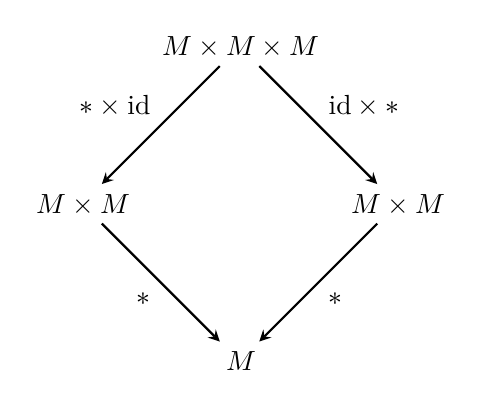
\begin{tikzpicture}[->,>=stealth,thick]
\node (A) at (0,0) {$M\times M\times M$};
\node (B) at (-2,-2) {$M\times M$};
\node (C) at (2,-2) {$M\times M$};
\node (D) at (0,-4) {$M$};

\draw (A) -- node[midway,above left]{$*\times \text{id}$} (B);
\draw (A) -- node[midway,above right]{$\text{id}\times *$} (C);
\draw (B) -- node[midway,below left]{$*$} (D);
\draw (C) -- node[midway,below right]{$*$} (D);
\end{tikzpicture}
\end{center}
\end{frame}


\begin{frame}{Remark}
\vspace{-0.2cm}
\begin{block}{Remark on Commutative (Abelian) Monoids.}  
A monoid \((M, *, e)\) consists of a set \(M\), a binary operation \(* : M \times M \to M\), and an identity element \(e\) satisfying:
\[
(a * b) * c = a * (b * c), \qquad e * a = a * e = a, \quad \forall a,b,c \in M.
\]

If, in addition, the operation \(*\) satisfies
\[
a * b = b * a, \quad \forall a,b \in M,
\]
then the monoid is called a \textbf{commutative monoid}, or equivalently, an \textbf{abelian monoid}.

\textbf{Intuition:}  
Commutativity means that the order in which elements are combined does not affect the result.  
In a commutative monoid, both the associative property and the commutative property coexist with an identity element.
\end{block}
\end{frame}

\begin{frame}{Remark}
\begin{block}{Examples:}
\begin{itemize}
  \item \((\mathbb{N}, +, 0)\): addition of natural numbers — commutative and associative with identity \(0\).
  \item \((\mathbb{R}, \times, 1)\): multiplication of real numbers — commutative with identity \(1\).
  \item \((\mathbb{Z}, +, 0)\): addition of integers — commutative with identity \(0\).
\end{itemize}

\textbf{Non-Example:}
\((M_{2\times2}(\mathbb{R}), \times, I_2)\) is a monoid because matrix multiplication is associative and \(I_2\) acts as the identity,  
but it is \emph{not commutative} in general, since for many matrices \(A,B\), \(AB \neq BA.\)

\textbf{Historical Note:}  
The term \emph{abelian} originates from Niels Henrik Abel, a 19th-century mathematician who first studied commutative algebraic structures.     
    \end{block}
\end{frame}


\begin{frame}{Examples of Monoids}
\begin{block}{}
    \begin{itemize}
  \item $(\mathbb{N}, +, 0)$ — additive monoid.
  \item $(\mathbb{N}, \times, 1)$ — multiplicative monoid.
  \item $(\mathbb{R}, \times, 1)$ — commutative monoid (but not group).
  \item $(M_{2\times2}(\mathbb{Z}), +, O)$ where $O$ is the zero matrix.
  \item $(M_{2\times2}(\mathbb{Z}), \times, I_2)$ where $I_2$ is identity matrix.
\end{itemize}
\end{block}

\begin{block}{Visualization}
\begin{center}
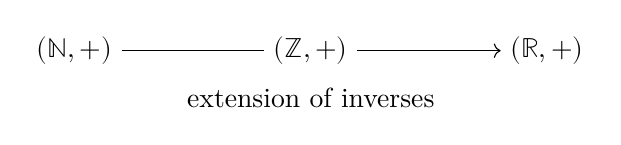
\begin{tikzpicture}
\node (N1) at (0,0) {$(\mathbb{N},+)$};
\node (Z1) at (3,0) {$(\mathbb{Z},+)$};
\node (R1) at (6,0) {$(\mathbb{R},+)$};
\draw[->] (N1)--(Z1)--(R1);
\node at (3,-0.6) {extension of inverses};
\end{tikzpicture}
\end{center}
\end{block}
\end{frame}


\begin{frame}{Equality of Left and Right Inverses}
\textbf{Proposition.}  
Let $(X, *, e)$ be a monoid, and let $a, b, c \in X$.  
If $b$ is a left inverse of $a$ and $c$ is a right inverse of $a$, i.e.
\[
b * a = e \quad \text{and} \quad a * c = e,
\]
then \(b = c\).  
Consequently, \(a\) is invertible and \(b=c=a^{-1}\).

\textbf{Proof.}
\[
b = b * e = b * (a * c) = (b * a) * c = e * c = c.
\]
Hence $b=c$, and both satisfy $a * b = b * a = e$.

\begin{block}{Conclusion}
In a monoid, if both left and right inverses exist for an element, they coincide.
\end{block}
\end{frame}

% ============================================================
\begin{frame}{Product of Invertible Elements}
\textbf{Proposition.}  
Let $(X, *, e)$ be a monoid.  
If $a,b \in X$ are invertible, then so is $a*b$.

\textbf{Proof.}
Let $a^{-1}$ and $b^{-1}$ denote their inverses:
\[
a * a^{-1} = e = a^{-1} * a, \quad b * b^{-1} = e = b^{-1} * b.
\]
Consider $(a*b) * (b^{-1} * a^{-1})$:
\[
(a*b) * (b^{-1} * a^{-1}) = a*(b*b^{-1})*a^{-1} = a*e*a^{-1} = a*a^{-1} = e.
\]
Similarly,
\[
(b^{-1} * a^{-1}) * (a*b) = b^{-1}*(a^{-1}*a)*b = b^{-1}*e*b = e.
\]
Thus $(b^{-1}*a^{-1})$ is the inverse of $(a*b)$.

\textbf{Hence:} The set of invertible elements in a monoid is closed under the binary operation.
\end{frame}

% ============================================================
\section{Groups}
% ============================================================

\begin{frame}{Definition of a Group}
\textbf{Definition.}  
A \emph{group} is a quadruple $(G, *, e, i)$ where
\begin{enumerate}
  \item $(G,*,e)$ is a monoid,
  \item For every $x\in G$, there exists an inverse $i(x)\in G$ such that
  \[
  x * i(x) = i(x) * x = e.
  \]
\end{enumerate}

\begin{block}{Remarks:}
\begin{itemize}
  \item The map $i:G\to G$ sending $x\mapsto i(x)$ is called the \emph{inverse map}.
  \item The group is called \emph{commutative} or \emph{abelian} if
  \[
  x*y = y*x, \quad \forall x,y\in G.
  \]
\end{itemize}
\end{block}

\end{frame}

% ============================================================
\begin{frame}{Examples of Groups}
\textbf{Examples:}
\begin{enumerate}
  \item $(\mathbb{Z}, +, 0, -)$  
        Abelian group under addition.  
        \(\forall x\in\mathbb{Z},\, x+(-x)=0.\)
  \item $(M_{n\times n}(\mathbb{Z}), +, O_n, -)$  
        Additive abelian group of integer matrices.
  \item $(M_{n\times n}(\mathbb{R}), +, O_n, -)$ and  
        $(M_{n\times n}(\mathbb{Q}), +, O_n, -)$  
        Additive abelian groups of real or rational matrices.
\end{enumerate}

\begin{center}
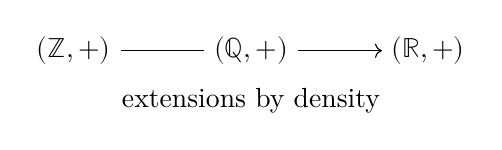
\begin{tikzpicture}[scale=0.9]
\node (Z) at (0,0) {$(\mathbb{Z},+)$};
\node (Q) at (2.5,0) {$(\mathbb{Q},+)$};
\node (R) at (5,0) {$(\mathbb{R},+)$};
\draw[->] (Z)--(Q)--(R);
\node at (2.5,-0.7) {extensions by density};
\end{tikzpicture}
\end{center}
All are \emph{abelian} since addition is commutative.
\end{frame}

% ============================================================
\section{Group of Units}
% ============================================================

\begin{frame}{Definition: Group of Units}
\begin{block}{Definition.}  
Let $(X, *, e)$ be a monoid.  
The set of all invertible elements of $X$ is denoted by
\[
X^* = \{\, x \in X \mid \exists\, x^{-1}\in X,\; x*x^{-1}=x^{-1}*x=e \,\}.
\]
This set forms a group under $*$, called the \textbf{group of units} of $X$.
\end{block}

\textbf{Proof (Sketch).}
\begin{itemize}
  \item Closure: proved earlier (product of invertibles is invertible).
  \item Associativity: inherited from the monoid.
  \item Identity: $e\in X^*$, $e^{-1}=e$.
  \item Inverse: each $x\in X^*$ has inverse $x^{-1}\in X^*$.
\end{itemize}
\end{frame}

% ============================================================
\begin{frame}{Examples of Groups of Units}
\begin{block}{Multiplicative Groups:}
\[
\begin{array}{lll}
(X, *, e) & X^* & \text{Reason}\\ \hline
(\mathbb{Z}, \times, 1) & \{-1,1\} & \text{only $\pm1$ have multiplicative inverses in $\mathbb{Z}$} \\
(\mathbb{Q}, \times, 1) & \mathbb{Q}\setminus\{0\} & \text{nonzero invertible} \\
(\mathbb{R}, \times, 1) & \mathbb{R}\setminus\{0\} & \text{nonzero invertible}
\end{array}
\]
\end{block}
\begin{block}{Additive/Other Groups:}
\[
\begin{array}{lll}
(\mathbb{N}, +, 0) & \{0\} & \text{identity only}\\
(\mathbb{N}, \times, 1) & \{1\} & \text{1 only}
\end{array}
\]
\end{block}
\end{frame}


\begin{frame}{Remark: Restriction of a Function}
Let $X, Y$ are two sets and \(f:X\to Y\) and \(U\subseteq X\).

\textbf{Definition.}
The \emph{restriction} of \(f\) to \(U\) is the function
\[
f|_U : U \to Y, \quad f|_U(x) = f(x)\text{ for }x\in U.
\]

\textbf{Remark.}
If \(U\subseteq V\subseteq X\), then
\[
(f|_V)|_U = f|_U.
\]

\centering
\begin{tikzpicture}[
    % Removed the problematic global arrow tip definition
    node distance=4em and 5em, % Defines separation distance (vertical and horizontal)
    every node/.style={inner sep=6pt} % Standard spacing for all nodes
]
    % 1. Define the nodes using explicit positioning
    \node (U) {$U$};
    % X is below U
    \node (X) [below=of U] {$X$};
    % Y is to the right of U
    \node (Y) [right=of U] {$Y$};
    
    % 2. Draw the arrows

    % U -> Y (Horizontal map f|_U)
    % Using the standard '->' arrow style, which is guaranteed to work
    \draw[->] (U) -- (Y)
        node[midway, above] {$f|_U$};

    % U -> X (Vertical map, using an explicit 'hook' style)
    % The original diagram used a 'hook' for this inclusion map.
    % We replace the standard '->' with 'right hook->' from the 'arrows' library
    \draw[right hook->] (U) -- (X);

    % X -> Y (Diagonal map f)
    \draw[->] (X) -- (Y)
        node[midway, below left] {$f$};

\end{tikzpicture}


\end{frame}

\begin{frame}{Remark: Shrink of a Function}
\textbf{Remark (Shrink).}  
Sometimes one considers a \emph{shrinking} of a function’s domain to a subset where a certain property holds (e.g., continuity, invertibility).

Formally, if \(P(x)\) is a property on \(X\), define
\[
\text{Shrink}_P(f) = f|_{\{x\in X \mid P(x)\text{ holds}\}}.
\]
Thus, a \emph{shrink} is a restricted version of \(f\) preserving only the portion of its domain where it satisfies a given property.
\end{frame}


\begin{frame}{General and Special Linear Groups}
\begin{block}{Definition (General Linear Group).}  
For a field \(F\) and integer \(n \ge 1\),
\[
GL_n(F) = \{ A \in M_{n\times n}(F) \mid \det(A) \ne 0 \}.
\]
Under matrix multiplication, \(GL_n(F)\) forms a group.\\
\textbf{Identity:} \(I_n\). \\
\textbf{Inverse:} \(A^{-1} = \frac{1}{\det(A)} \operatorname{adj}(A)\).

\end{block}



\begin{block}{Definition (Special Linear Group).}
\[
SL_n(F) = \{ A \in GL_n(F) \mid \det(A) = 1 \}.
\]
It is a normal subgroup of \(GL_n(F)\).
\end{block}
\end{frame}

\begin{frame}{Relation Between $\mathbf{GL_n}$ and $\mathbf{SL_n}$}
\begin{center}
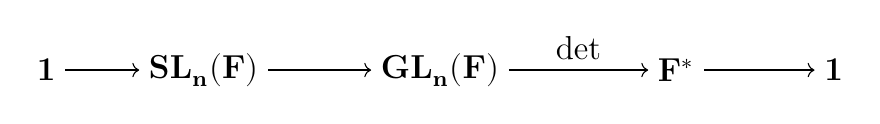
\begin{tikzpicture}[scale=1.0, every node/.style={font=\large}]
% Define the nodes
\node (one) at (-4, 0) {$\mathbf{1}$};
\node (sl) at (-2, 0) {$\mathbf{SL_n(F)}$};
\node (gl) at (1, 0) {$\mathbf{GL_n(F)}$};
\node (f) at (4, 0) {$\mathbf{F^*}$};
\node (one2) at (6, 0) {$\mathbf{1}$};

% Draw the maps
% 1 to SL_n (Trivial map / inclusion)
\draw[->] (one) -- (sl);

% SL_n to GL_n (Inclusion map) - this is the injective part (\rightarrowtail is common for injective)
\draw[->] (sl) -- (gl);

% GL_n to F^* (Determinant map) - this is the surjective part
\draw[->] (gl) -- node[above] {$\det$} (f);

% F^* to 1 (Trivial map)
\draw[->] (f) -- (one2);
\end{tikzpicture}

\vspace{1.5cm} % Space between diagram and text

% The textual exact sequence
\begin{block}{Short Exact Sequence}
\begin{equation*}
1 \to SL_n(F) \to GL_n(F) \xrightarrow{\det} F^* \to 1
\end{equation*}
\end{block}

\end{center}

\alert{Interpretation:} $\mathbf{SL_n(F)}$ (matrices with determinant 1) is the \textbf{kernel} of the determinant map, making it a normal subgroup of $\mathbf{GL_n(F)}$. The quotient group $\mathbf{GL_n(F)} / \mathbf{SL_n(F)}$ is isomorphic to $\mathbf{F^*}$, the multiplicative group of the field $F$.
\end{frame}

% ============================================================
\section{Function Composition and Monoids}
% ============================================================

\begin{frame}{Proposition on Composition of Functions}
Let \(A,B,C,D\) be sets and let  
\(f:A\to B,\; g:B\to C,\; h:C\to D.\)

\begin{block}{Proposition.}
\[
h \circ (g \circ f) = (h \circ g) \circ f.
\]
That is, function composition is associative.
\end{block}

\textbf{Proof.}
For all \(x\in A\),
\[
[h \circ (g \circ f)](x) = h(g(f(x))) = [(h \circ g) \circ f](x).
\]
Therefore both sides define the same function.

\begin{block}{Consequences}
Function composition forms a monoid operation on the set of all maps from a set to itself.
\end{block}
\end{frame}

\begin{frame}{Corollary: The Function Monoid}
\begin{block}{Corollary.}
Let \(A\) be a set.  
Then \((\text{End}(A), \circ, \mathrm{id}_A)\) is a monoid,  
where \(\text{End}(A) = \{ f : A \to A \}\).
\end{block}

\textbf{Proof.}
\begin{itemize}
  \item Composition is associative (previous proposition).
  \item Identity function acts as neutral element: \(f\circ\mathrm{id}_A = \mathrm{id}_A\circ f = f.\)
\end{itemize}
Hence it satisfies monoid axioms. \(\square\)
\end{frame}

% ============================================================
\section{Groups of Bijections and Permutations}
% ============================================================

\begin{frame}{Definition: Group of Bijections}
\begin{block}{Automorphisms}
    The set of all bijections \(f:A\to A\) under composition forms a group,  
denoted by \(\mathrm{Aut}(A)\) or \(S_A\), called the \emph{group of automorphisms (permutations)} of \(A\).

\textbf{Properties:}
\begin{itemize}
  \item Closure: composition of bijections is bijection.
  \item Associativity: inherited from function composition.
  \item Identity: \(\mathrm{id}_A\).
  \item Inverse: each bijection has inverse function.
\end{itemize}
\end{block}
\end{frame}

% ============================================================
\begin{frame}{Permutation Group \(S_n\)}
\begin{block}{Definition.}
For a finite set \(A=\{1,2,\dots,n\}\),
\[
S_n = \{ \text{all bijections } A \to A \}
\]
is called the \emph{symmetric group on $n$ letters}.  
\(|S_n| = n!\).
\end{block}

\begin{block}{Notation:} permutations often written in two-line form:
\[
\sigma = \begin{pmatrix}
1 & 2 & 3 \\
2 & 3 & 1
\end{pmatrix}
\quad \text{means } \sigma(1)=2,\ \sigma(2)=3,\ \sigma(3)=1.
\]
\end{block}
\end{frame}

% ============================================================
\begin{frame}{Example: The Group \(S_3\)}
Elements of \(S_3\):
\[
\begin{array}{lcl}
\text{identity:} & e = (1)(2)(3), \\
\text{transpositions:} & (12), (13), (23),\\
\text{3-cycles:} & (123), (132).
\end{array}
\]

\textbf{Non-commutativity Example:}
\[
(12)\circ(23) = (123), \quad (23)\circ(12) = (132),
\]
and \((123) \ne (132)\).  
Hence \(S_3\) is \textbf{not commutative} (non-abelian).

\begin{center}
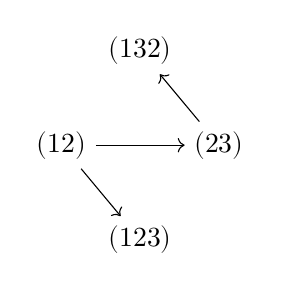
\begin{tikzpicture}[node distance=1cm]
\node (a) at (0,0) {$(12)$};
\node (b) at (2,0) {$(23)$};
\node (ab) at (1,-1.2) {$(123)$};
\node (ba) at (1,1.2) {$(132)$};
\draw[->] (a)--(b);
\draw[->] (a)--(ab);
\draw[->] (b)--(ba);
\end{tikzpicture}
\end{center}
\end{frame}

% ============================================================
\begin{frame}{Summary}
\begin{itemize}
  \item Proved equality of left and right inverses and closure of invertibles.
  \item Defined groups, abelian groups, and examples.
  \item Introduced the group of units \(X^*\).
  \item Defined \(GL_n(F)\), \(SL_n(F)\) with exact-sequence relation.
  \item Proved associativity of composition, showed \((\text{End}(A),\circ)\) monoid.
  \item Defined groups of bijections and permutation groups \(S_n\), with \(S_3\) as first non-abelian example.
  \item Clarified restriction and shrink remarks for functions.
\end{itemize}
\end{frame}

\begin{frame}{Thanks}
  \cmcendframe
\end{frame}

\end{document}
